\documentclass[fontset=none]{ctexart}

\setCJKmainfont{SimSun}
\setmonofont{DejaVu Sans Mono}
% Latin Modern

\setcounter{tocdepth}{5}
\setcounter{secnumdepth}{5}
% -1 part
% 0 chapter
% 1 section
% 2 subsection
% 3 subsubsection
% 4 paragraph
% 5 subparagraph

\usepackage{cite}
\usepackage{geometry}
\geometry{a4paper,scale=0.7}

\usepackage{algorithm}  
\usepackage{algorithmicx}  
\usepackage{algpseudocode}
\makeatletter
\newenvironment{breakablealgorithm}
  {% \begin{breakablealgorithm}
   \begin{center}
     \refstepcounter{algorithm}% New algorithm
     \hrule height.8pt depth0pt \kern2pt% \@fs@pre for \@fs@ruled
     \renewcommand{\caption}[2][\relax]{% Make a new \caption
       {\raggedright\textbf{\ALG@name~\thealgorithm} ##2\par}%
       \ifx\relax##1\relax % #1 is \relax
         \addcontentsline{loa}{algorithm}{\protect\numberline{\thealgorithm}##2}%
       \else % #1 is not \relax
         \addcontentsline{loa}{algorithm}{\protect\numberline{\thealgorithm}##1}%
       \fi
       \kern2pt\hrule\kern2pt
     }
  }{% \end{breakablealgorithm}
     \kern2pt\hrule\relax% \@fs@post for \@fs@ruled
   \end{center}
  }
\makeatother

\usepackage{amsmath}
\usepackage{amssymb}
\usepackage{graphicx}
\usepackage{subfigure}
\usepackage{changepage}
\usepackage{multirow}
\usepackage{url}

\usepackage{amsthm}
\newtheorem{theorem}{Theorem}[section]
\newtheorem{lemma}[theorem]{Lemma}
\newtheorem{proposition}[theorem]{Proposition}
\newtheorem{corollary}[theorem]{Corollary}
% \newtheorem{remark}{Remark}[section]
\newtheorem{example}{Example}[section]
\newenvironment{solution}{\begin{proof}[Solution]}{\end{proof}}
\theoremstyle{definition}
\newtheorem{definition}{Definition}[section]
\theoremstyle{remark}
\newtheorem*{remark}{Remark}

\usepackage[colorlinks, linkcolor=black, citecolor=blue, bookmarksnumbered]{hyperref}
% \hypersetup{
% 	colorlinks=true,
% 	linkcolor=cyan,
% 	filecolor=blue,      
% 	urlcolor=red,
% 	citecolor=green,
% }

\usepackage{fancyhdr}
\pagestyle{fancy}
\renewcommand{\sectionmark}[1]{\markright{\thesection\ #1}}
\fancyhf{}
\cfoot{\thepage}
\lhead{\rightmark}
% \rightmark 当前的节名
% \leftmark 当前的章名
% \(l/c/r)head{}, \(l/c/r)foot{}
\renewcommand{\headrulewidth}{0.4pt}
\renewcommand{\footrulewidth}{0pt}

\renewcommand\refname{References}
\renewcommand\contentsname{Content}
\renewcommand\figurename{Figure}

\begin{document}

\begin{titlepage}
    \begin{center}
        \vspace*{1cm}
            
        \Huge
        \textbf{Traffic Predicion With Advanced Graph Neural Networks}
            
        \vspace{0.5cm}
        \LARGE
        Mid-term Report\\
            
        \vspace{1.5cm}
            
        \textbf{11812804}  董\quad 正\\
        \textbf{11813225}  王宇辰\\
        \textbf{11811305}  崔俞崧\\

        \vspace{0.5cm}
        Supervisior: 宋轩
            
        \vfill
            
        
\includegraphics[width=\textwidth]{images/sustc.png}
            
        \vspace{0.2cm}
            
        \Large
        Department of Computer Science and Engineering\\
        \vspace{0.5cm}
        Dec. 2020
            
    \end{center}
\end{titlepage}

\tableofcontents

\clearpage
\section{Preliminaries}
\subsection{Review}
\subsubsection{TTE}
\textbf{Travel Time Estimation (TTE)} is one of the most important researching topic in the traffic forecasting field. 
Estimating the travel time of any path in a city is of great importance to traffic monitoring, route planning, ridesharing, taxi dispatching, etc.
On Sep. 2020, DeepMind published a blog named \textit{Traffic prediction with advanced Graph Neural Networks}. 
This blog briefly described the whole industrial structure of estimated times of arrival (ETAs) techniques applied in Google Map but did not given any detailed implementation or any code.
Our work is based on the model structure of TTE proposed in the blog.
\begin{figure}[htb]
    \centering
    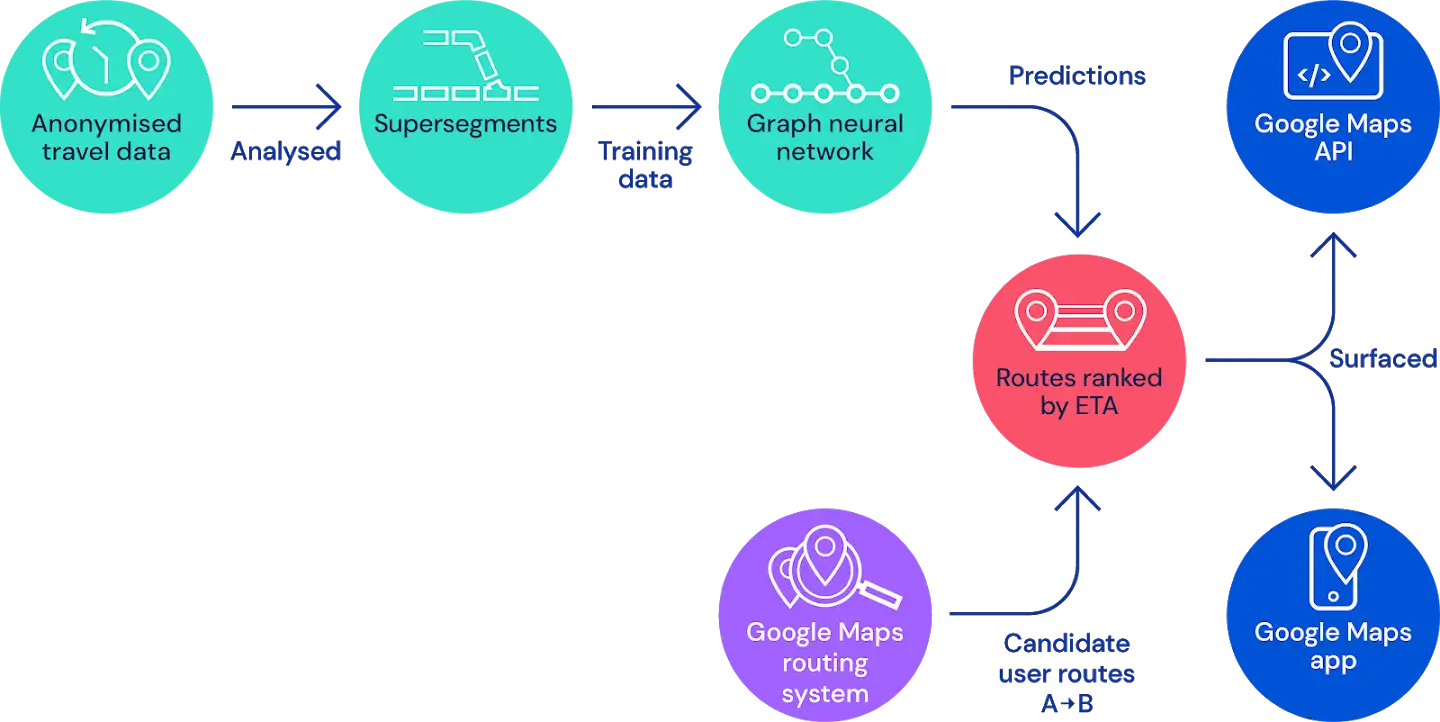
\includegraphics[width=0.9\textwidth]{images/architecture.png}
    \caption{Architecture}
    \label{fig1}
\end{figure}

\subsubsection{Goal}
Our ultimate goal (tentative) is to implement the industrial structure and apply it to the open source databases in China, then compare the performance with the state-of-the-art structures and find its application value.
This semester, we will first learn about the relative algorithms. More specifically, the two main algorithm we will use: TTE algorithm and Graph Neural Network (GNN). After that, we will learn the methods of processing traffic data. Finally, we combine the algorithms and apply them on some open source database.

\subsection{Introduction}
In the last stage, we stated the basic ideas of two state-of-the-art algorithms named \textit{DeepTTE}
and \textit{DCRNN}. As for this month, we have got some open source data and learned how to process the
data. What's more, we got deep in the code of \textit{DeepTTE} and researched on a new concept
called \textbf{Travel Time Index (TTI)}. And we also researched on the \textit{Supersegment} and proposed
a new computing process.

Breifly, we will state our work in this report as:
\begin{itemize}
    \item Implementation of \textit{DeepTTE} by 王宇辰
    \item Travel Time Index by 崔俞崧
    \item A Research on Supersegment by 董正
\end{itemize}

\section{Implementation of DeepTTE}
Three parts of implementation is mentioned below. First is dataset, gives the basic information of data composition to analysis. Second is algorithm, gives the structure and algorithm in the procedure of implement. Third is result, gives loss after training and loss in testing.\cite{wang2018when}
\subsection{Dataset}
Basic infos driverID, dateID (the date in a month, from 0 to 30), weekID (the day of week, from 0 to 6 (Mon to Sun)), timeID (the ID of the start time (in minute), from 0 to 1439), dist (total distance of the path (KM)), time (total travel time (min), i.e., the ground truth. You can set it as any value during the test phase)
Trip info for each node in one time:
\begin{itemize}
  \item states: the sequence of taxi states (available/unavaible)
  \item lngs: the sequence of longitutes of all sampled GPS points
  \item lats: the sequence of latitudes of all sampled GPS points
  \item time\_gap: Each value indicates the time gap from current point to the firt point
  \item dist\_gap: Each value indicates the dist gap from current point to the firt point
\end{itemize}
Statistic info as mean value and standard deviation of trip infos.

\subsection{Algorithm}
The alogrithm is applied with Pytorch. Using ConvolutionNN and RecurrentNN structures.
In Attribute Component only mix personal info, without use complex models. In Spatio-Temporal Component, it is dived into two parts, first is the Geo-Conv layer using ConvolutionNN model, second is beyond the layer, using LSTM model, a kind of RecurrentNN. In Multi-Task Component, mainly using error functions to estimate the model. The Entire Estimator uses rooted mean squared error and mean absolute error, and the Local Estimator uses mean absolute percentage error and only apllied in training. Also, in training, the two estimator is weighted combined.
\begin{figure}[htb]
  \centering
  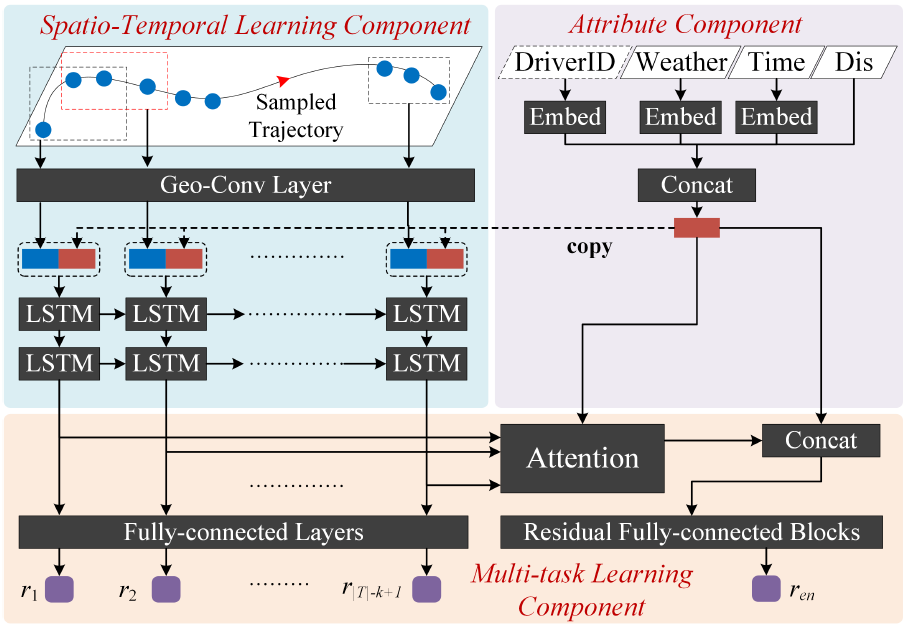
\includegraphics[width=\textwidth]{images/deepTTEstruct.png}
  \caption{Model}
  \label{fig: DeepTTEstuct}
\end{figure}

\subsection{Result}
The result contains two columns, the first is real time of time travel, the second is predict time of time travel.
% \begin{figure}[htb]
%   \centering
%   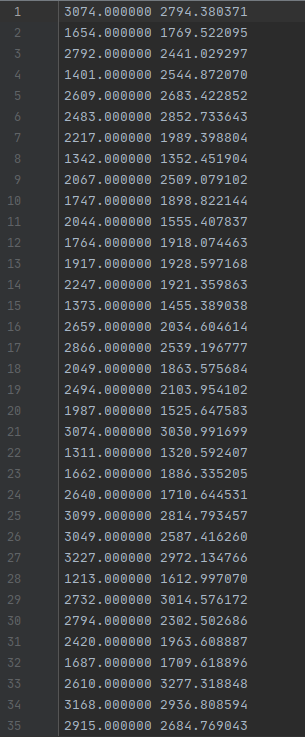
\includegraphics[width=0.5\textwidth]{images/deepTTEres.png}
%   \caption{Result}
%   \label{fig: DeepTTEres}
% \end{figure}
\begin{verbatim}
  3074.000000 2794.380371
  1654.000000 1769.522095
  2792.000000 2441.029297
  1401.000000 2544.872070
  2609.000000 2683.422852
  2483.000000 2852.733643
  2217.000000 1989.398804
  1342.000000 1352.451904
  2067.000000 2509.079102
  1747.000000 1898.822144
  2044.000000 1555.407837
  1764.000000 1918.074463
  1917.000000 1928.597168
  2247.000000 1921.359863
  1373.000000 1455.389038
  2659.000000 2034.604614
  2866.000000 2539.196777
  2049.000000 1863.575684
  2494.000000 2103.954102
  1987.000000 1525.647583
  3074.000000 3030.991699
  ...
\end{verbatim}
The training contains 100 epoches.
\begin{figure}[h]
  \centering
  \subfigure[Epoch 1] {
    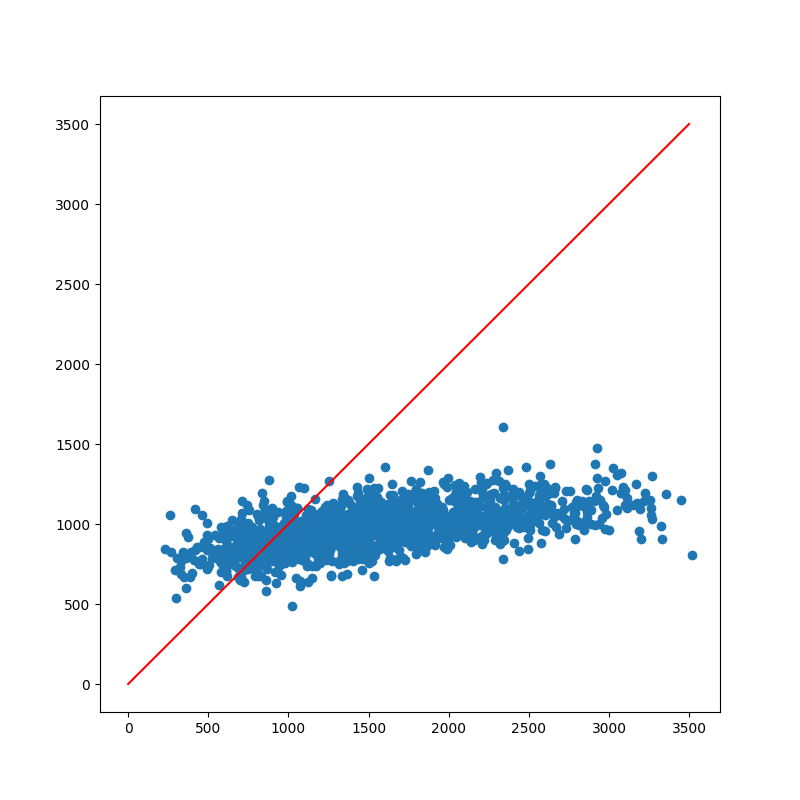
\includegraphics[width=0.25\textwidth]{images/ep1.png}
  }
  \quad
  \subfigure[Epoch 5] {
    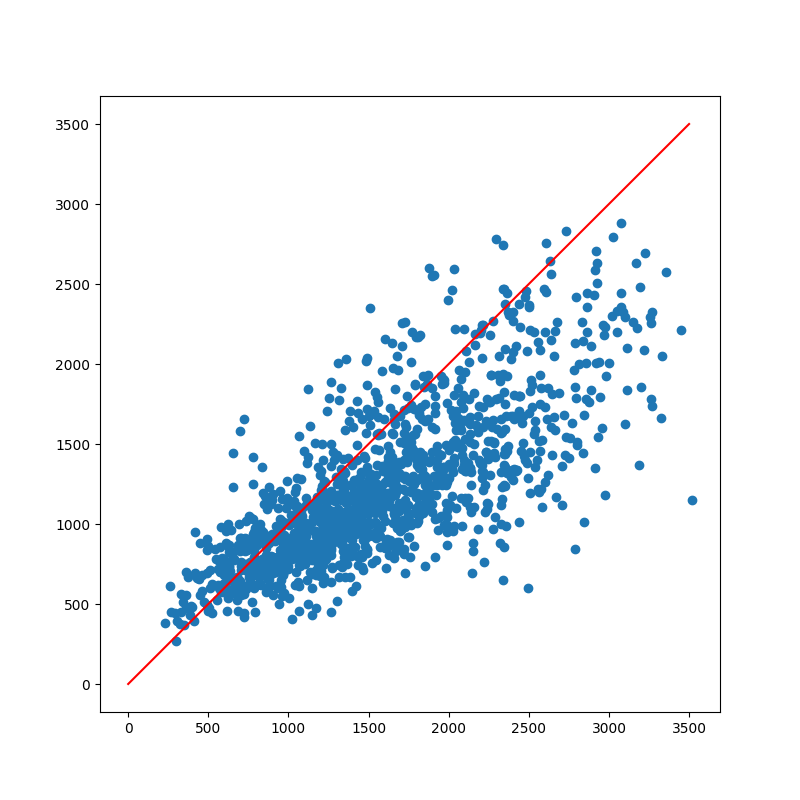
\includegraphics[width=0.25\textwidth]{images/ep5.png}
  }
  \quad
  \subfigure[Epoch 100] {
    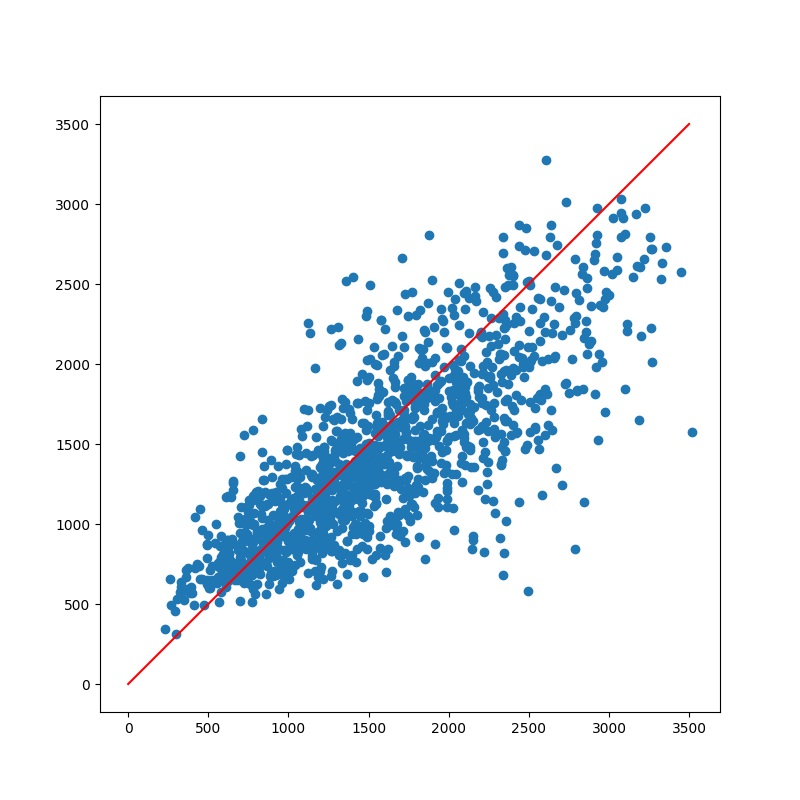
\includegraphics[width=0.25\textwidth]{images/ep100.png}
  }
  \caption{Training Epochs}
  \label{fig: deepTTEepochs}
\end{figure}
\clearpage
From above, the result is close to the function $y=x$, shows that the result is accurate to estimate the real time. Also, with line chart below, we can see that, error in training is rather low, about 0.02 after training, and testing on the test set, the error is about 0.2, it is a good result in travel time estimation.
\begin{figure}[htb]
  \centering
  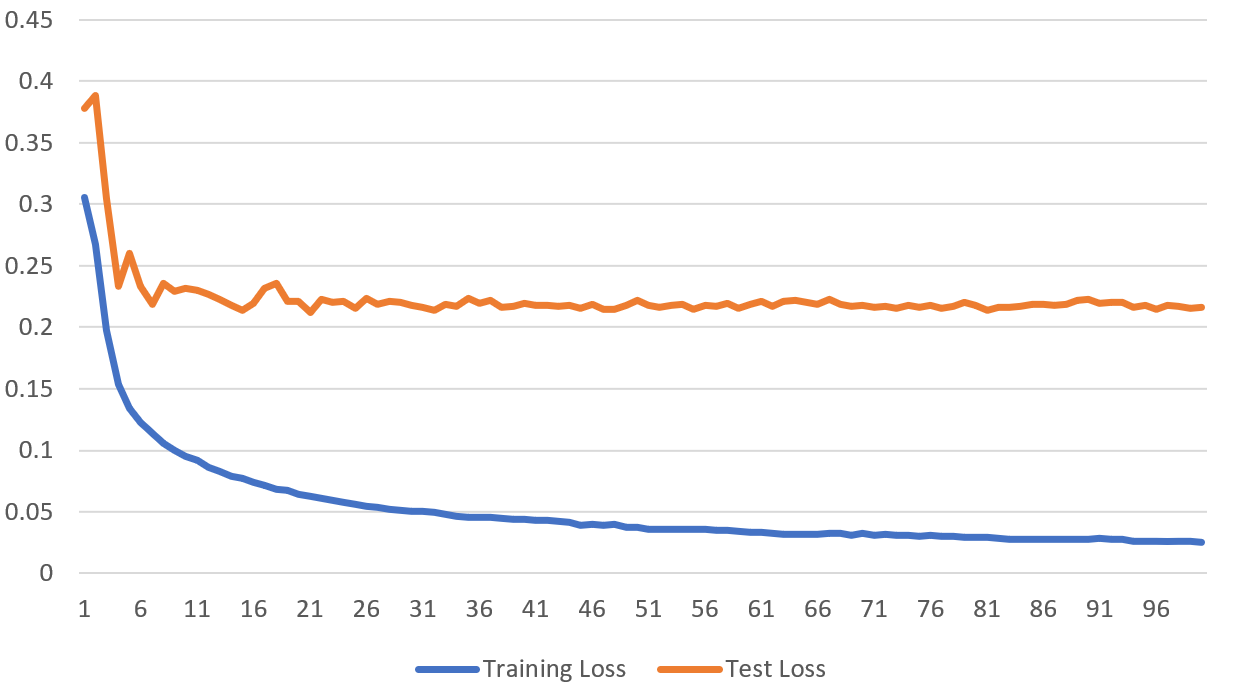
\includegraphics[width=\textwidth]{images/loss.png}
  \caption{Loss}
  \label{fig: DeepTTEloss}
\end{figure}

\clearpage
\section{Travel Time Index}
\subsection{Introduction}
The \textbf{TTI (Travel Time Index)} industry's most used evaluation index of urban congestion degree is the ratio of the actual travel time and the free flow time. The larger the value, the worse the traffic operation status, and the congestion level is generally positive. Related, other abnormal weather conditions (such as rain, snow, fog, etc.) or abnormal road conditions may also affect the value of TTI.
\begin{figure}[htb]
  \centering
  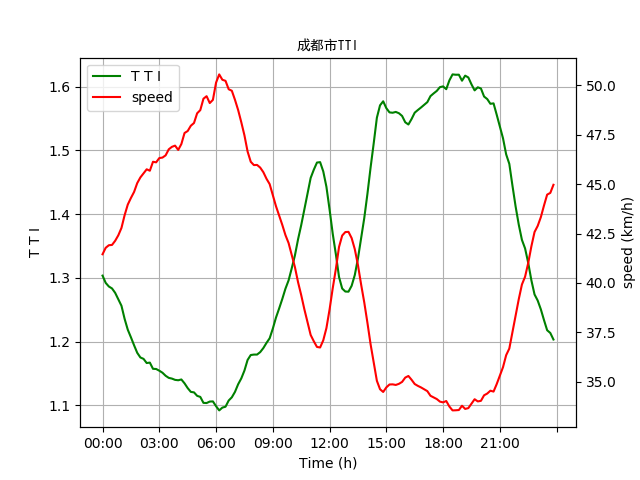
\includegraphics[width=\textwidth]{images/chengdutti.png}
  \caption{TTI Data Curves of Chengdu}
  \label{fig: ttieg}
\end{figure}

\subsection{Basic Idea}
The basic idea of Speed: If a link has two time slices, $t_1$ and $t_2$, and the link's length is $S$, then the average speed $v$ of the link is: $v = 2S / (t_1 + t_2)$ during the period from $t_1$ to $t_2$.

The basic idea of TTI: In the same link in a time slice, $TTI = free\ flow\ speed / actual\ speed$.

\subsection{Calculation}
\begin{equation}
  TTI=\frac{\sum_{i=1}^N\frac{L_i}{V_i}\cdot W_i}{\sum_{i=1}^N\frac{L_i}{V_{free\_i}}\cdot W_i} \notag
\end{equation}
\begin{itemize}
  \item $L_i$: length of the road
  \item $W_i$: weight of road
  \item $V_i$: real time traffic information
  \item $V_{free\_i}$: free flow velocity
\end{itemize}

\subsection{Motivation}
The reasons for TTI calculation are as follows:

DeepTTE algorithm has some shortcomings:
\begin{enumerate}
  \item Excessively strict requirements on data. The input of DeepTTE algorithm is trajectory data, which is usually unstable, the requirements of the algorithm are very strict. In the data preprocessing stage, the interval point of trajectory data should be between 200-400m and should not be too large. In addition, the data used in the demonstration of the paper are all selected and processed.
  \item The effect is not stable enough. There are various problems such as excessive error and data loss in trajectory data, and the results obtained by using such data for training will be too deviated from the ideal.
  \item There is a certain distance from academia to industry. In industrial applications, the trajectory data obtained is quite different from the data set used in this paper, and the results obtained when directly used as input are not ideal due to the lack of data and errors.
  The purpose of TTI calculation is to improve DeepTTE algorithm and change the input data from the original track data to the road TTI data. TTI data has the advantages of more stable and smaller error. Since TTI data is calculated through the trajectory data, the calculation process is the first step of the processing of the trajectory data, so that the TTI data has a smaller error than the trajectory data.  
\end{enumerate}

\subsection{Dataset}
\begin{itemize}
    \item Data source: Didi Chuxing GAIA Intiative
    \item Region: Chengdu
    \item Time: 2018-10-01 to 2018-12-01
    \item Content:
        \begin{itemize}
            \item GPS track of taxis with timestamps
            \item Coordinate of road and district boundaries
            \item TTI and average speed of districts
        \end{itemize}
\end{itemize}
\begin{figure}[htb]
  \centering
  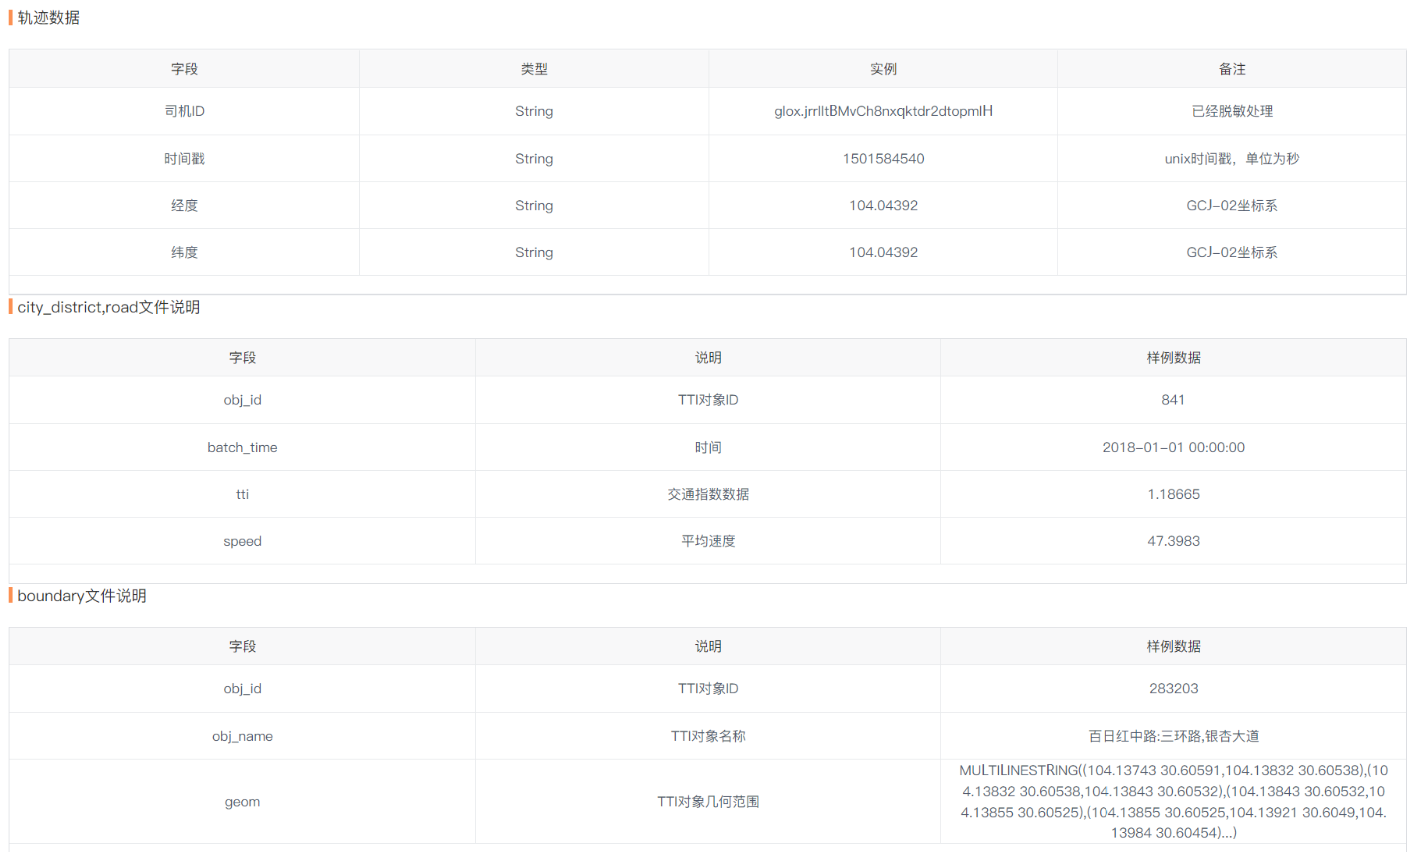
\includegraphics[width=\textwidth]{images/chengdudata.png}
  \caption{Dataset}
  \label{fig: ttidata}
\end{figure}

\subsection{Data Processing and TTI Computing Method}
It can be seen from the calculation formula of TTI that the key to calculating TTI is to get each feature in the following table, which are road network data, real-time traffic data, free flow data and weight data.

The road network data and real-time traffic data can be obtained directly from the data set, while the free flow data and weight data need to be extracted from the data set by using some methods.
The extraction method of free flow data is as follows: since free flow is defined as the traffic flow information when there is no congestion, the traffic flow information located at 2:00-5:00 am can be selected as the free flow information since this is the time when congestion is least likely to occur.
Extraction method of weight data: the number of vehicles passing through each section in a month is counted and recorded, and this number is the weight data.
After processing the data information, the TTI calculation formula can be used to calculate the TTI data of each road.
\begin{table}[h]
  \begin{tabular}{|c|p{0.7\textwidth}|}
    \hline
    \textbf{Feature} & \textbf{Detail}\\
    \hline
    Road network data & Basic map road network data, including road shape and unique id\\
    \hline
    Realtime Traffic data & Relying on dripping massive floating car data, real-time traffic data released by Didi\\
    \hline
    Free flow data & From the Drip Trajectory database, the road speed generated by the excavation\\
    \hline
    Weight data & The total number of vehicles passing the road within a natural month\\
    \hline
  \end{tabular}
\end{table}

\clearpage
\section{Supersegment}
\subsection{Introduction}
\textbf{Supersegment} is a new concept proposed in a blog by \textit{DeepMind}.
But unfortunately, \textit{DeepMind} did not give any formal definition. Instead, they stated that
``We divided road networks into `Supersegments' consisting of multiple adjacent segments of road that share significant traffic volume.''\cite{blog}

As for my understanding, Supersegment is a division of road that the adjacent segments have something
in common such as speed and volume, but at the same time, there are also differences that big enough
to distinguish them.

\subsection{Dataset}
\begin{itemize}
    \item Data source: Didi Chuxing GAIA Intiative
    \item Region: Chengdu
    \item Time: 2018-10-01 to 2018-12-01
    \item Content:
        \begin{itemize}
            \item GPS track of taxis with timestamps
            \item Coordinate of road and district boundaries
            \item TTI and average speed of districts
        \end{itemize}
\end{itemize}
\begin{figure}[htb]
  \centering
  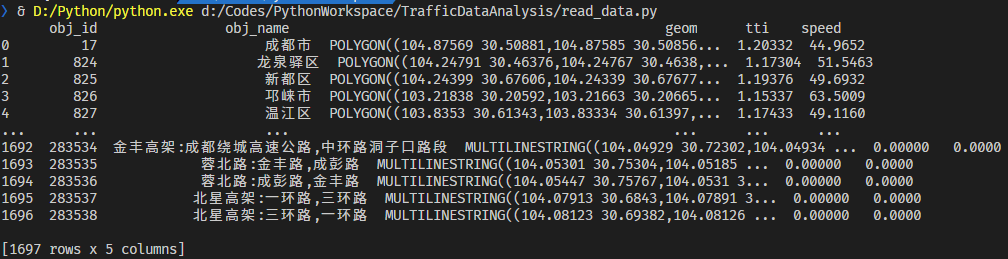
\includegraphics[width=\textwidth]{images/dataset.png}
  \caption{Data}
  \label{fig: dataset}
\end{figure}

\subsection{Problem Description}
Currently, there is no algorithm of Supersegment or ``road division''. 
Therefore, I need to work on myself.

Now, we have
\begin{itemize}
    \item Coordinate of road boundaries
    \item GPS data of taxis
    \item Timestamps
\end{itemize}
And we need to work out a partition of a road.
\begin{figure}[htb]
    \centering
    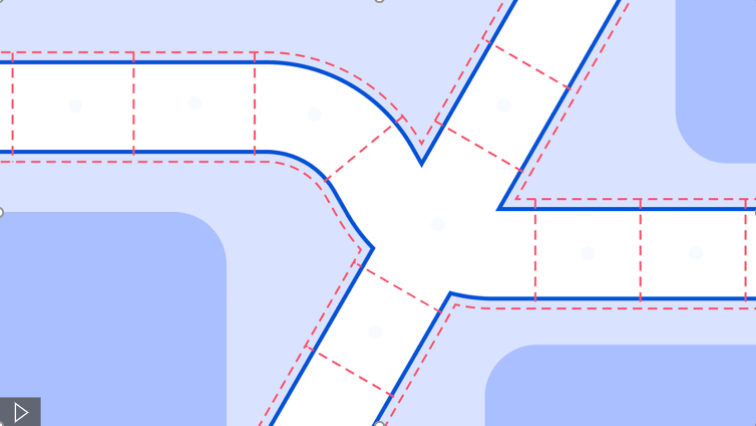
\includegraphics[width=0.5\textwidth]{images/supersegment.png}
    \caption{Supersegments}
    \label{fig: supersegment}
\end{figure}

\subsection{Model Design}
In this section, I will propose a model to compute Supersegments.
At the very first, I need to ensure that I will base on \textbf{speed} to do the division.
There is a three-step approach of my design:
\begin{enumerate}
    \item Locate GPS coordinates of taxis into corresponding roads
    \item Use the timestamps to calculate average speed and regead it as the instantaneous speed of midpoint
    \item Apply clustering algorithm to these midpoints
\end{enumerate}

First, since we know the boundaries of the roads, we can determine the coordinate is on which road.
After that, we draw the GPS points on the road. Because we know the timestamp of each point, we can 
calculate the average speed of two adjacent points and just consider it as the speed of their midpoint.
Note that the closer the points are, the closer the average speed is to the actual instantaneous speed.
So the best way is to select adjacent points if our data is abundant.
\begin{figure}[htb]
  \centering
  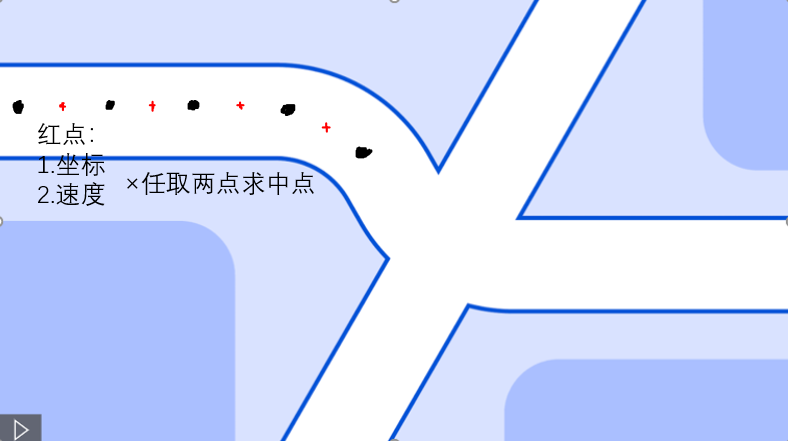
\includegraphics[width=0.9\textwidth]{images/midpoints.png}
  \caption{Find the midpoints}
  \label{fig: midpoint}
\end{figure}

Next step is to apply clustering algorithm like \textit{K-Means} to find a certain number of clusters
of the midpoints.
Every midpoint has three features:
\begin{itemize}
  \item longitude
  \item latitude
  \item speed
\end{itemize}

So actually this is a three-dimension clustering, but the result we need is two-dimensional, which means
we need to balance the weight of these features carefully to get a correct partition.
And finally, these clusters give us segments.
% \begin{figure}[htb]
%   \centering
%   \begin{minipage}[t]{0.48\textwidth}
%     \centering
%     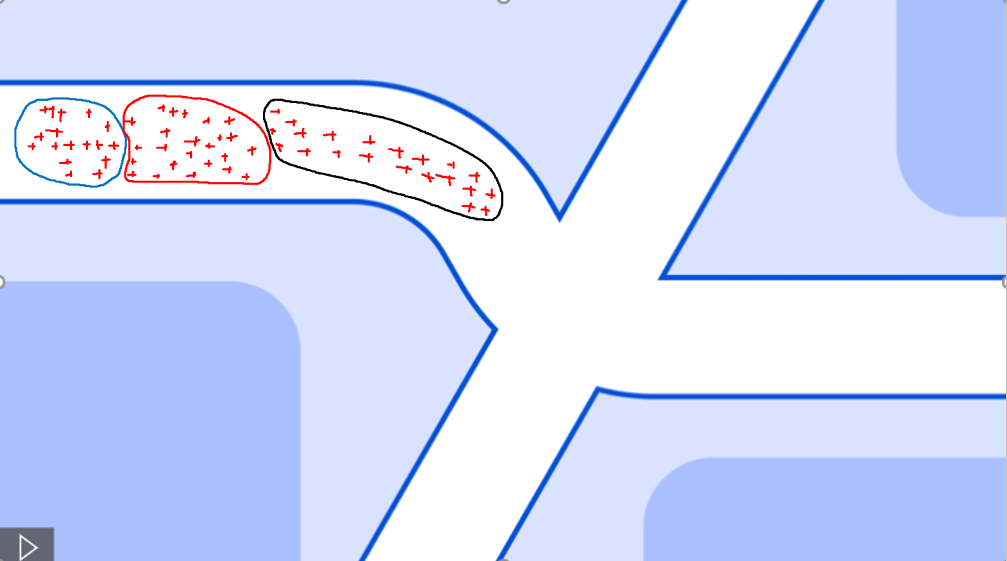
\includegraphics[width=0.45\textwidth]{images/cluster.png}
%     \caption{Clusters}
%     \label{fig: cluster}
%   \end{minipage}
%   \begin{minipage}[t]{0.48\textwidth}
%     \centering
%     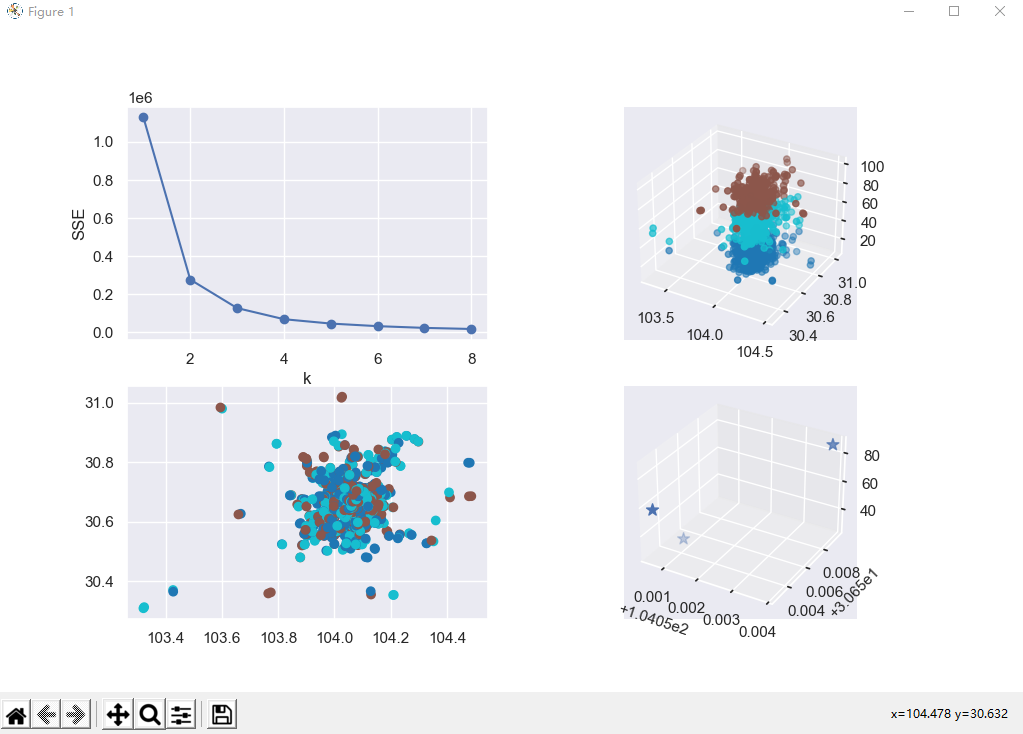
\includegraphics[width=0.45\textwidth]{images/kmeans.png}
%     \caption{K-Means}
%     \label{fig: cluster}
%   \end{minipage}
% \end{figure}

\begin{figure}[h]
  \centering
  \subfigure[Clusters] {
    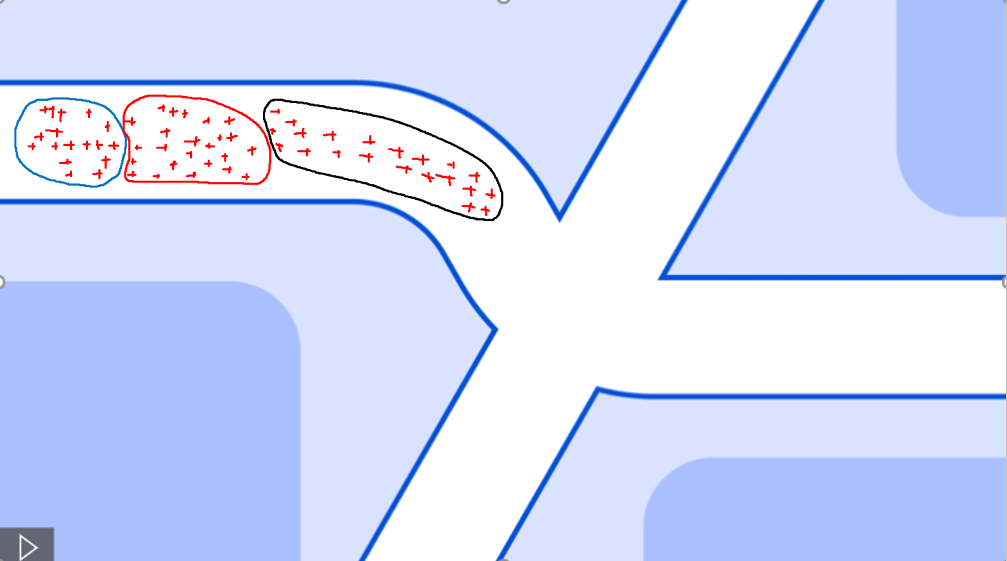
\includegraphics[width=0.45\textwidth]{images/cluster.png}
  }
  \quad
  \subfigure[K-Means Example] {
    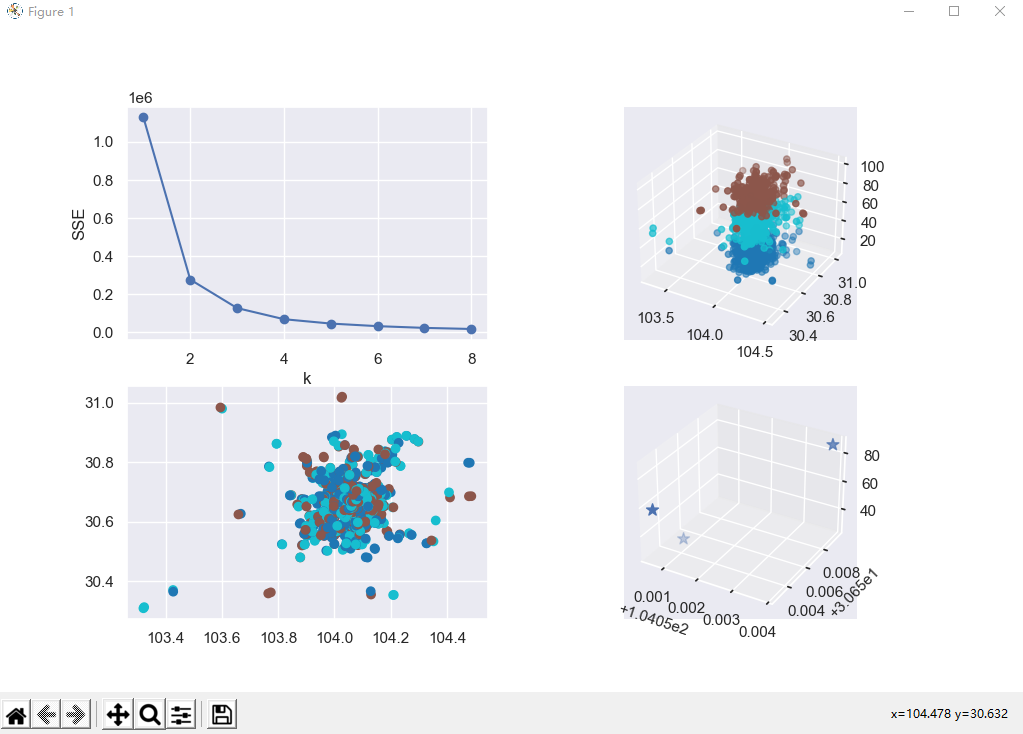
\includegraphics[width=0.45\textwidth]{images/kmeans.png}
  }
\end{figure}

\subsection{Conclusion}
While it is just my personal thought, there are still many problems that are hard to handle.
One vital task is how to evaluate a Supersegment division is good. I do not have any idea.
And I still do not know whether \textit{K-Means} algorithm will work well on this topic.
But anyway, I think my model is at least feasible and I will continue researching on it if given more time.

\clearpage
\phantomsection
\addcontentsline{toc}{section}{References}
\bibliographystyle{ieeetr}
\bibliography{references}

\end{document}